\clearpage

\begin{figure}[p]
    \centering
    
\includegraphics[width=\linewidth]{/Users/jacekdmochowski/PROJECTS/fus_bold/figures/tFUS_Figure1.png}
    \caption{ 
    \textbf{Experimental overview.} 
    \textbf{(a)} MRI-compatible setup for transcranial focused ultrasound stimulation (tFUS) during 3 T resting-state fMRI. A circular transducer is secured to the forehead with an elastic headband to target the (right) subgenual anterior cingulate cortex (sgACC). Participants ($N = 16$) completed two counterbalanced sessions (Active, Sham) spaced two weeks apart. \textbf{(b)} Sagittal MRI slice highlighting the location of the sgACC. 
    \textbf{(c)} Empirical beampattern measured in a water tank (500 kHz carrier) showing lateral spread and focal depth (i.e., approximately 6 cm); free-field spatial-peak temporal-average intensity $I_{\mathrm{spta}}=667\,\mathrm{mW/cm^2}$. 
    \textbf{(d)} Session timeline: a 15-min BOLD acquisition was divided into three 5-min windows (Pre, tFUS, Post). In Active sessions, sonication occurred only in the middle window.
    \textbf{(e)} One-minute zoom of the stimulation train used during the tFUS window: five cycles of 20 s ON / 40 s OFF; within ON-epochs, pulses were delivered at 40 Hz and 30\% duty. 
    \textbf{(f)} Analysis pipeline: data were preprocessed with fMRIPrep; sgACC-centered functional connectivity (FC; Fisher-z correlations to all parcels) was computed per subject, condition, and window. The prespecified primary test was a subject-level linear mixed-effects model with fixed effects for time, condition, and their interaction, evaluating the Pre to Post difference-in-differences (DiD, Active-Sham, Post-Pre).
    }
    \label{fig:process_figure}
\end{figure}

\begin{figure}[p]
    \centering
    
\includegraphics[width=\linewidth]{/Users/jacekdmochowski/PROJECTS/fus_bold/figures/fc_change_vs_fc_baseline_violin_plot.png}
    \caption{\textbf{tFUS increases connectivity of the sgACC after Active but not Sham stimulation.}
    \textbf{(a)} \emph{Sham tFUS.} Scatter-overlaid bar plots show the distribution of sgACC–whole-brain FC at each window (Pre, tFUS, Post);  markers denote subject means and thin lines connect subjects across time. FC remains stable across time, consistent with the results of the mixed‐effects model (tFUS vs.\ pre: $\beta=-0.020$, $p=0.444$; post vs.\ pre: $\beta=-0.011$, $p=0.671$).
    \textbf{(b)} \emph{Active tFUS.} The same visualization reveals a ``ramping'' trajectory from baseline through post-sonication.  The difference-in-differences ($\Delta FC_{\mathrm{Active}} - \Delta FC_{\mathrm{Sham}}$) is significantly positive after sonication (Active–Sham, Pre$\rightarrow$Post: $\beta=0.079$, 95$\%$ CI $[0.006,\,0.151]$, $p=0.033$), indicating a stimulation-specific increase in sgACC FC. A similar, smaller trend is present during tFUS (Pre$\rightarrow$tFUS interaction: $\beta=0.060$, $p=0.104$)
    \textbf{(c)} \emph{Baseline‐referenced connectivity change during tFUS.} Bars show subject-level means of $\Delta\mathrm{FC}=\mathrm{FC}_{\mathrm{tFUS}}-\mathrm{FC}_{\mathrm{Pre}}$ (error bars depict 95$\%$ CI). A planned post‐hoc contrast of Active versus Sham shows a trend towards a greater increase in FC during Active stimulation (Active–Sham $\Delta\mathrm{FC}=+0.060$, $p=0.051$).
    \textbf{(d)} \emph{Baseline‐referenced connectivity change post‐sonication.} Same as (c) but now shown for the post-sonication period: $\Delta\mathrm{FC}=\mathrm{FC}_{\mathrm{Post}}-\mathrm{FC}_{\mathrm{Pre}}$. The corresponding post‐hoc contrast is significant (Active–Sham $\Delta\mathrm{FC}=+0.079$, 95\% CI $[0.006,\,0.151]$, $p=0.034$).}


    \label{fig:sgacc_violin_2panel}
\end{figure}

\begin{figure}[p]
    \centering
    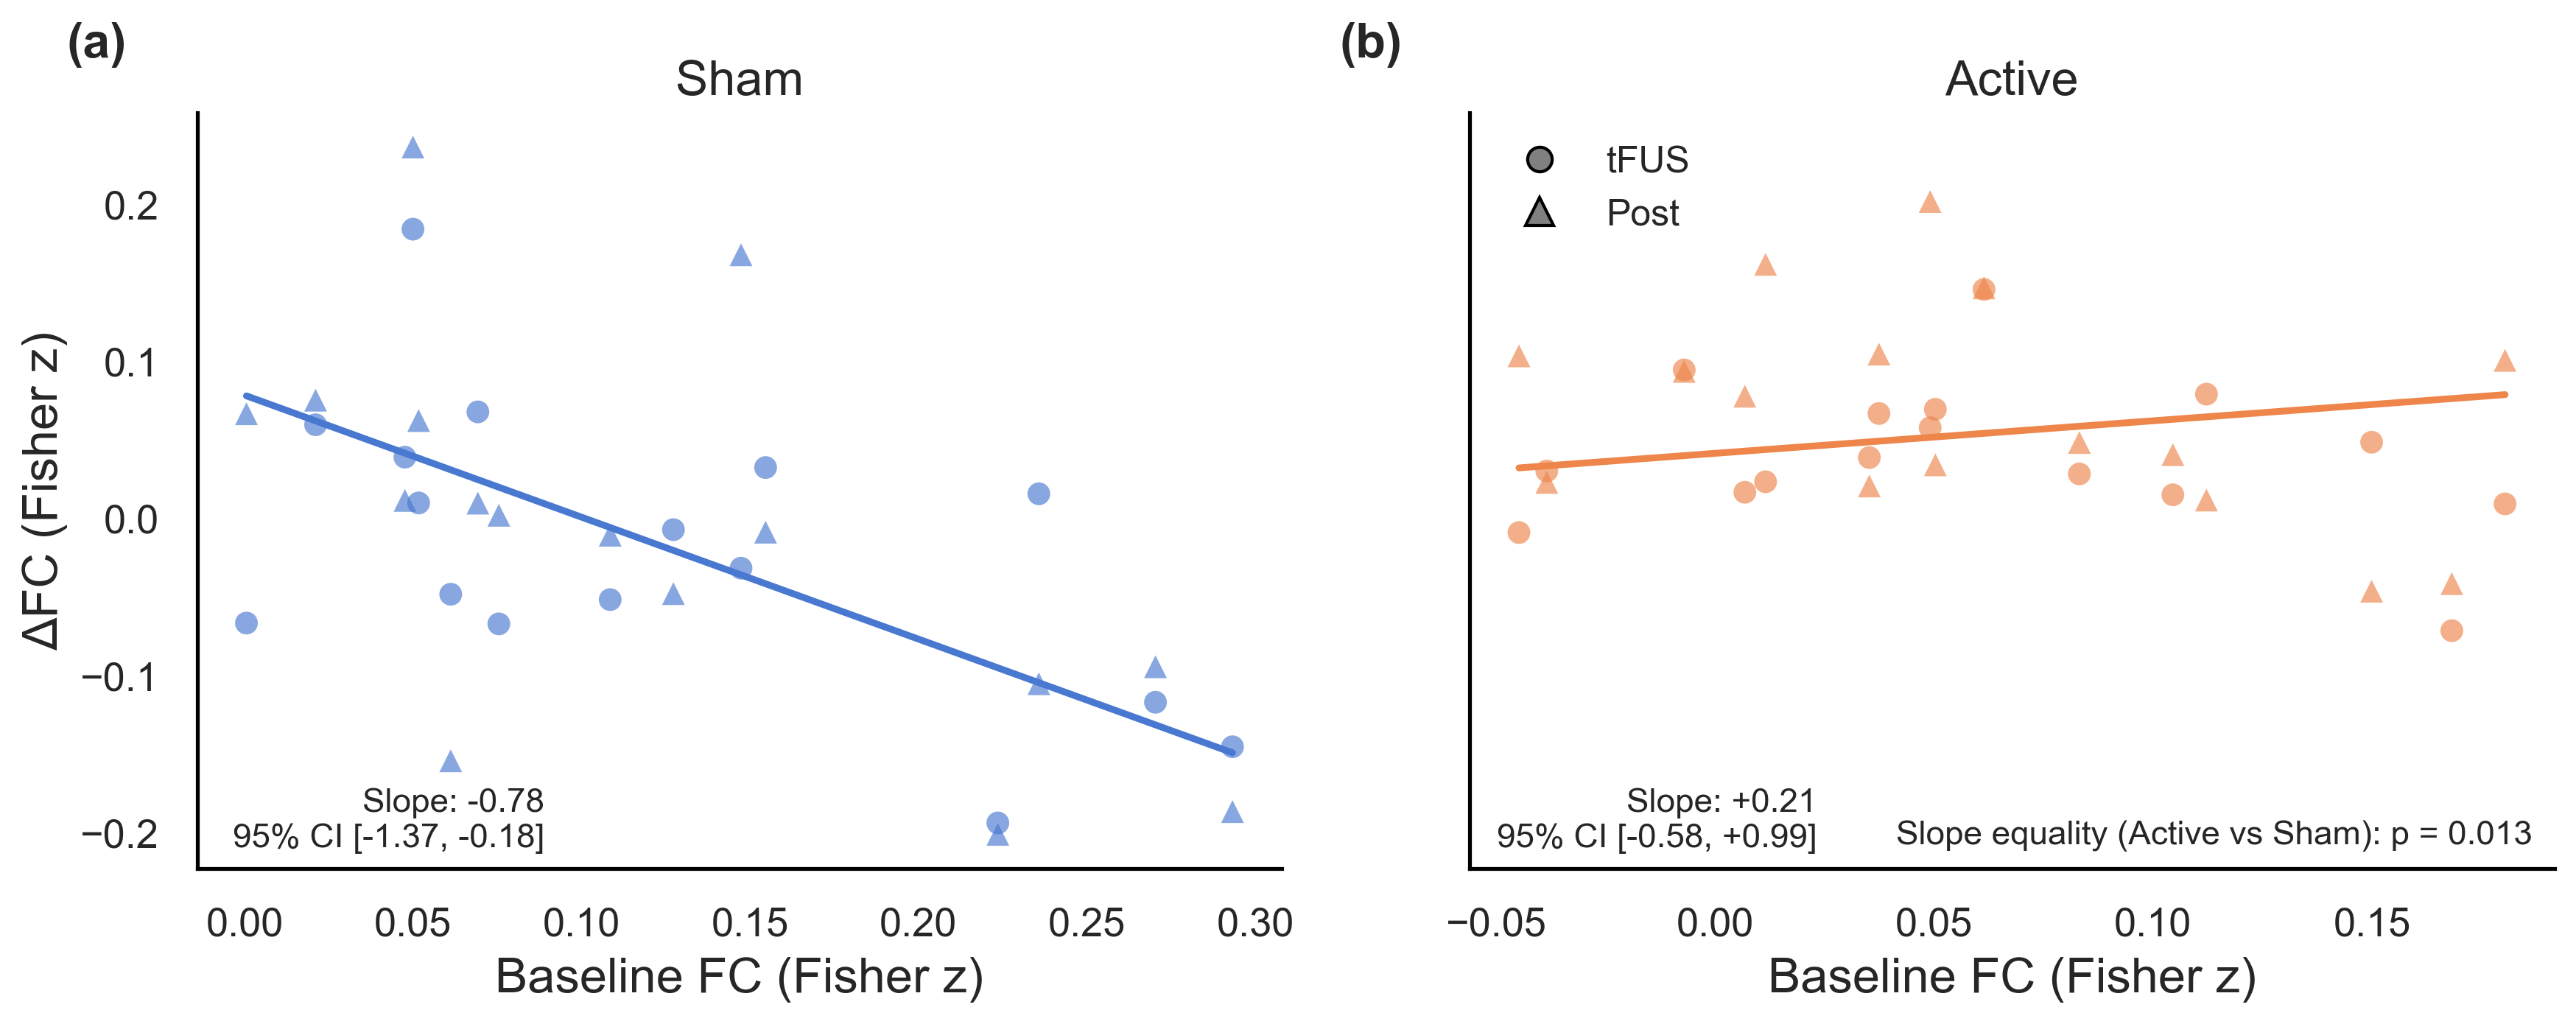
\includegraphics[width=\linewidth]{../figures/rtm_slope_pooled_2panel.png}
    \caption{\textbf{Baseline connectivity level predicts FC change in Sham but not Active tFUS.} (a) Sham tFUS: subject-level scatter of baseline sgACC FC (x-axis) versus change from baseline $\Delta\mathrm{FC}=\mathrm{FC}_{t}-\mathrm{FC}{\mathrm{pre}}$ (y-axis), with data pooled across tFUS $(\circ)$ and post-sonication $(\triangle)$ windows. The regression line is derived from an OLS model with fixed effects for subject, time-window, and condition. The inverse relationship between $\Delta$ FC and baseline FC observed in the Sham condition is consistent with a regression-to-the-mean account. 
    (b) Same as (a) but now shown for Active tFUS. The slope of the regression line is mildly positive and does not differ significantly from zero. Importantly, the difference in slopes between Active and Sham is significant ($p=0.013$), indicating that baseline effects are not driving the observed post-sonication connectivity increase during Active stimulation.}
    \label{fig:rtm_slope_pooled_2panel}
\end{figure}

\begin{figure}[p]
    \centering
    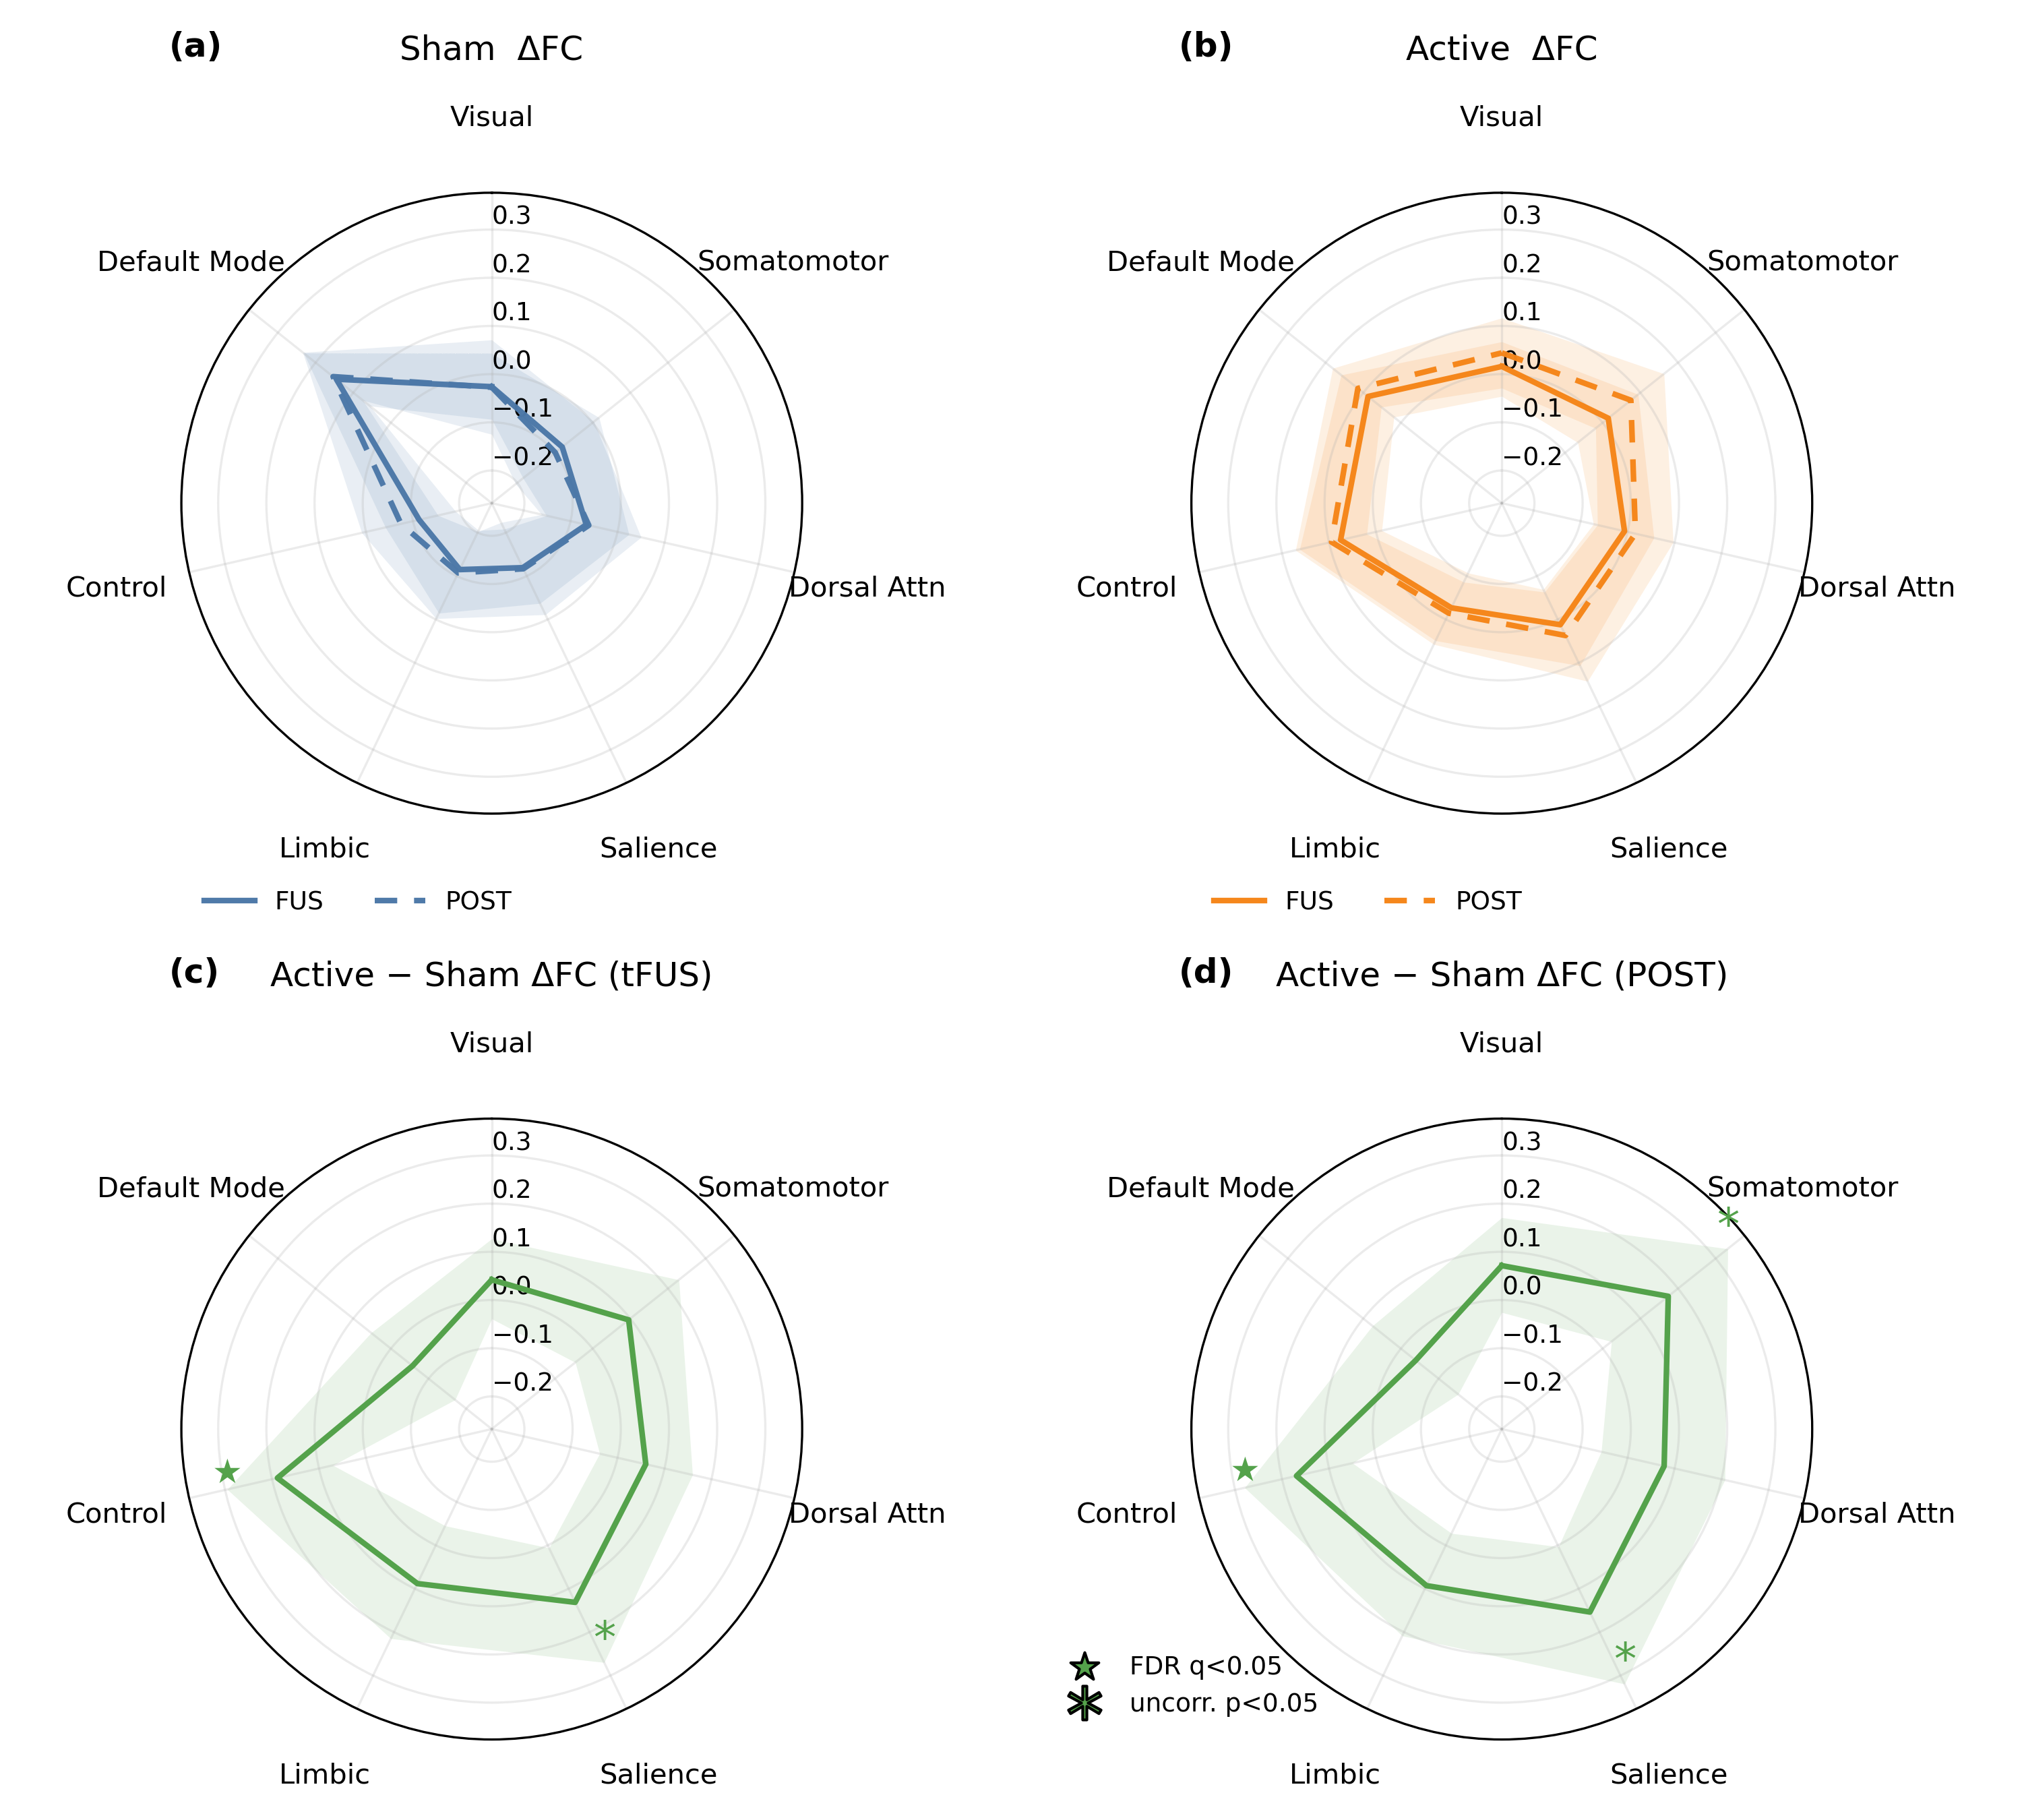
\includegraphics[width=\linewidth]{../figures/network_level_specificity_polar.png}
    \caption{\textbf{Network specificity of the sgACC connectivity increase under Active tFUS.}
    (a) \emph{Sham sessions:} baseline-referenced changes ($\Delta$FC) in sgACC coupling with the Yeo-7 networks indicate that the sgACC's connectivity with the Default Mode Network (DMN) increases over the course of the 15 minute recording (\texttt{tFUS}: solid; \texttt{Post}: dashed). 
    (b) \emph{Active tFUS:} In contrast, $\Delta$FC exhibits a more uniform pattern across the 7 canonical networks, with the largest increase observed at the Cognitive Control network.
    (c--d) \emph{Active--Sham differences in $\Delta$FC} shown at \texttt{tFUS} (c) and \texttt{Post} (d). Symbols mark directional tests ($H_1:\ \Delta\mathrm{FC}_{\text{active}}>\Delta\mathrm{FC}_{\text{sham}}$) corrected across networks using FDR: 
    filled star \raisebox{0.2ex}{\scriptsize$\star$}, $q<0.05$; asterisk \raisebox{0.2ex}{\scriptsize*}, uncorrected $p<0.05$. 
    At \texttt{tFUS}, the Cognitive Control network's coupling with the sgACC is significantly positive (FDR $q=0.028$), with the Salience network showing a positive trend (uncorr.\ $p=0.026$, $q=0.077$). 
    At \texttt{Post}, the Cognitive Control network's coupling remains elevated ($q=0.028$), while the Salience and Somatomotor networks exhibit trend-level, positive differences (Salience $q=0.077$; Somatomotor $q=0.066$). This data is consistent with a redistribution of sgACC coupling from the DMN toward task-positive networks (Control, Salience, Somatomotor) under Active stimulation.}
    \label{fig:network_level_specificity}
\end{figure}

\begin{figure}[p]
    \centering
    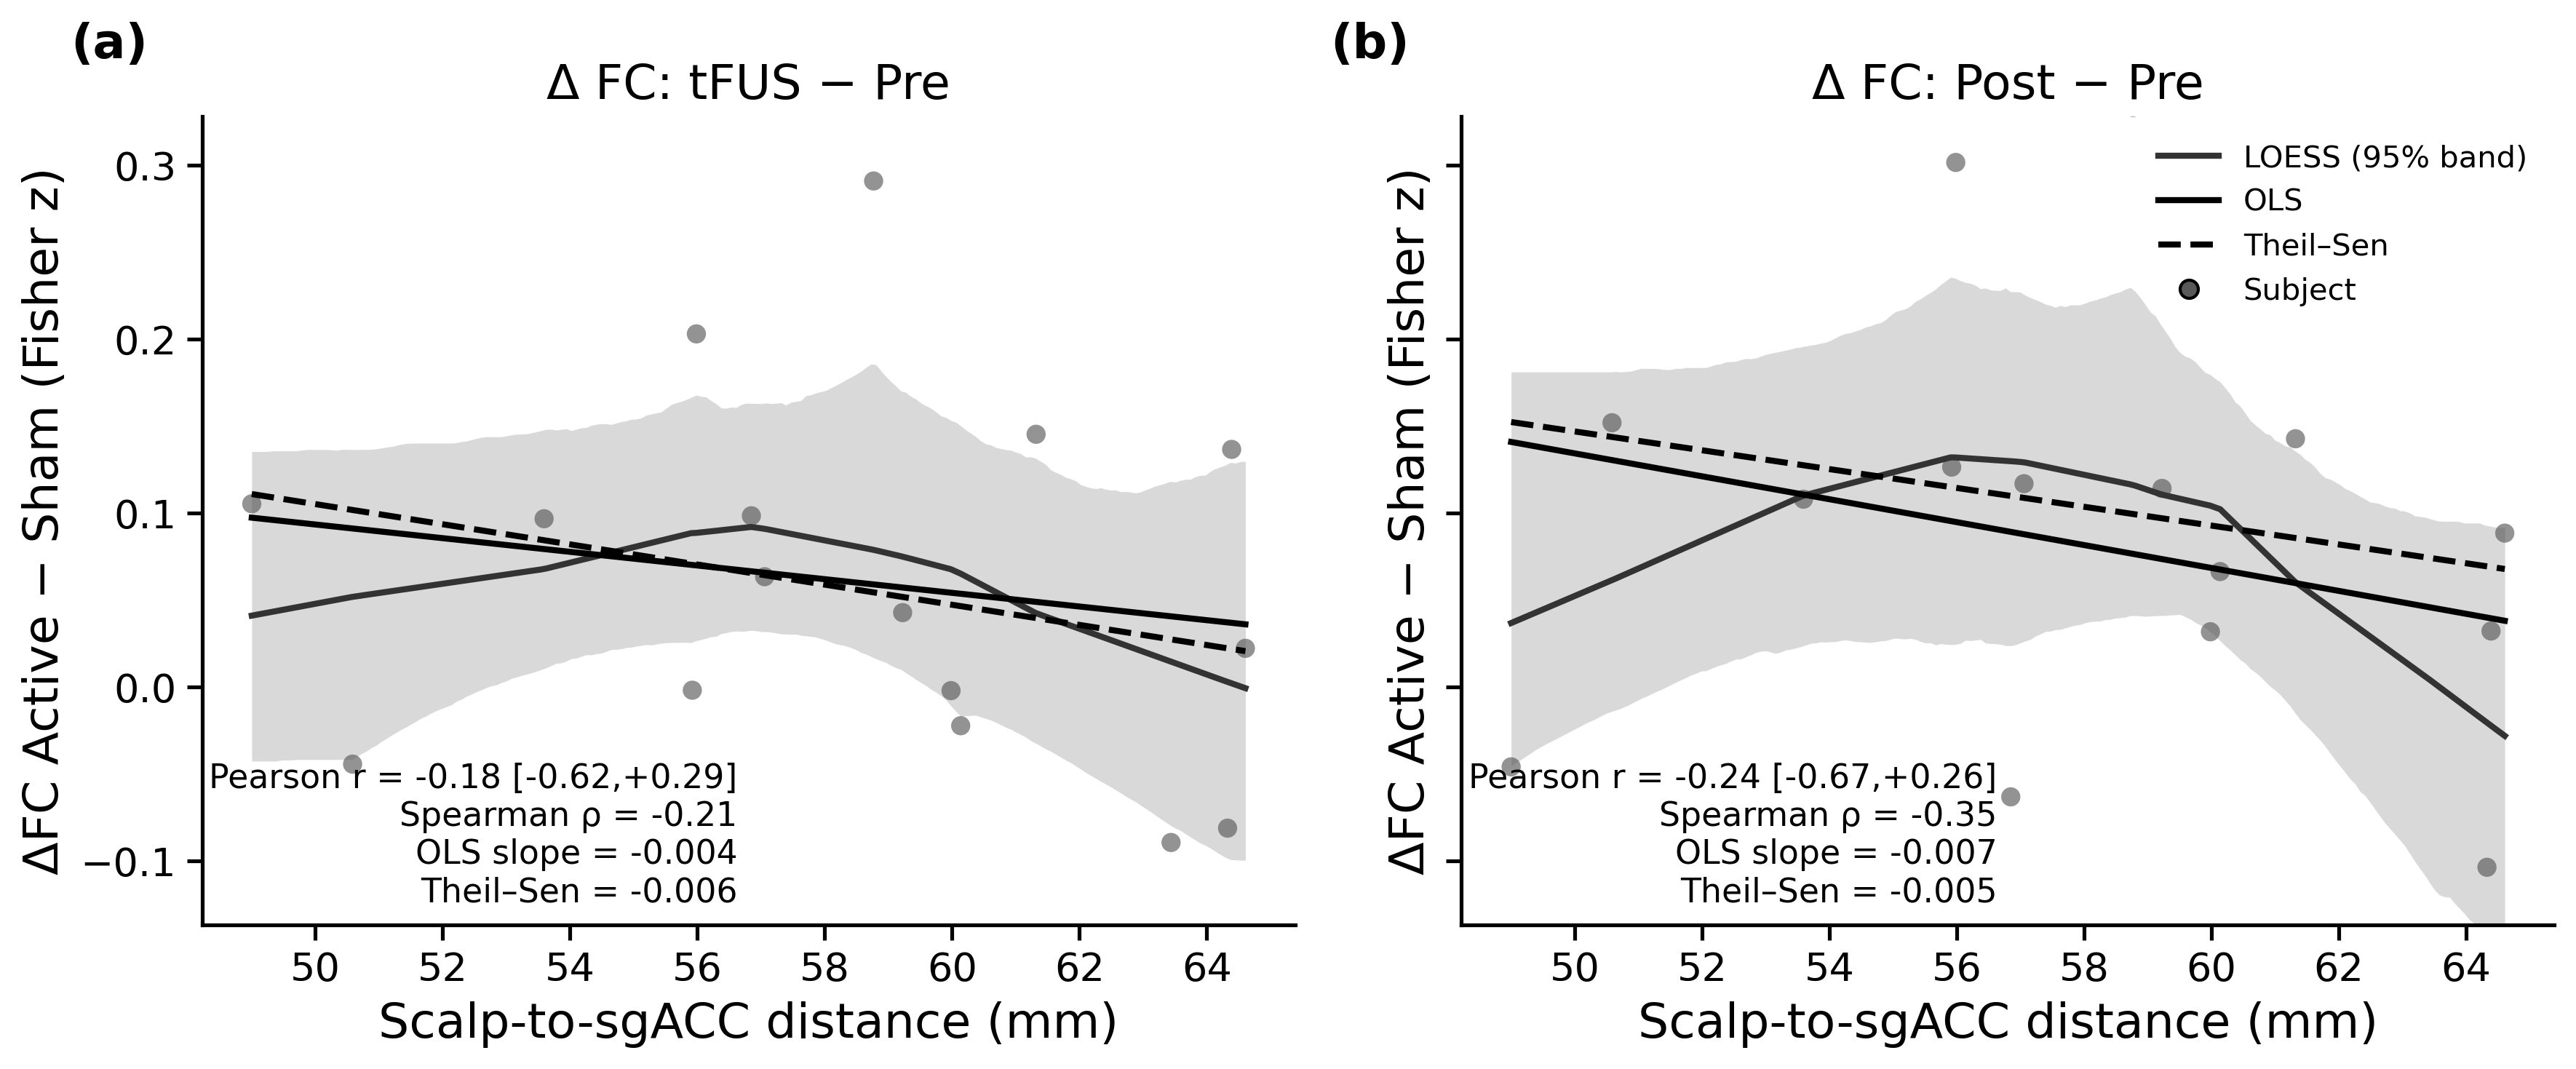
\includegraphics[width=\linewidth]{../figures/distance_vs_deltafc_loess_2panel.png}
    \caption{\textbf{Scalp--to--sgACC distance versus change in connectivity.} Panels show subject-level scatter of distance (mm) against $\Delta\mathrm{FC}$ (Fisher $z$ units) for the (a) tFUS and (b) Post-tFUS windows. Each panel overlays a LOESS smoother with a bootstrapped 95\% confidence interval (2{,}000 resamples), a least-squares regression line (solid), and a Theil--Sen robust regression line (dashed). The Post-tFUS panel exhibits a modest inverse trend, visually consistent with a dose-attenuation account; however, the moderation of the Post-tFUS effect by distance falls short of significance in the mixed-effects analysis ($p=0.083$).}
    \label{fig:distance_loess}
\end{figure}
